\documentclass[spanish]{beamer}
\usetheme{naked}
\mode<presentation>
\useoutertheme{miniframes}
\setbeamercolor{alerted text}{fg=cyan}

\usepackage[scaled=0.8]{beramono}
\usepackage{droidsans}

% \usefonttheme{professionalfonts}
% \usepackage{lmodern}
% \usepackage{arev}
% \usepackage{eucal}

\usepackage{tikz}
\usetikzlibrary{calc,3d}
\usepackage{tkz-berge}
%\usepackage{tkz-berge-add}
\usepackage{graphiso}

\usepackage{mathabx}
\usepackage{amsmath}

\usepackage[T1]{fontenc}
\usepackage[utf8]{inputenc}

\usepackage{booktabs}

\usepackage{minted}

\newcommand{\gen}[1]{{\langle #1\rangle}}
\newcommand{\setof}[2]{\left\{\,#1\mid #2\,\right\}}
\newcommand{\RR}{\mathbb{R}}

\newcommand{\graphcaption}[4][gray!80!white]{\draw (#2,#3) node [fill=#1]{#4};}

\renewcommand{\(}{\bigl(}
\renewcommand{\)}{\bigr)}

\DeclareMathOperator{\diam}{diam}
\DeclareMathOperator{\rec}{rec}

\newtheorem{teorema}{Teorema}
\newtheorem{proposicion}{Proposición}
\newtheorem{corolario}{Corolario}
\newtheorem{conjetura}{Conjetura}

\theoremstyle{definition}
\newtheorem{definiciones}{Definiciones}
\newtheorem{definicion}{Definición}
\newtheorem{ejemplo}{Ejemplo}

\SetVertexNotLabeledSmall
\tikzstyle{EdgeStyle}= [very thick]
\SetVertexSimple[FillColor=gray,MinSize=2pt]
\renewcommand*{\VertexLineWidth}{1pt}

\newcommand{\MVert}[3]{\VertexM[xa=#1,ya=#2,xb=4*cos(360*#3/24),
  yb=4*sin(360*#3/24),shows=1,starts=3,stops=16]{a#3}}
\newcommand{\MEdge}[3][60]{\EdgeM[bendsfrom=#1,shows=2,starts=3,stops=16]{a#2}{a#3}}

\newcommand{\MVerte}[3]{%
  % for some reason, the expresions have to be put in a macro before
  % being used as value of xa, ya. This did not happened with xb,
  % yb. Go figure.
  \pgfmathsetmacro{\thexa}{4*cos(36*#3)}
  \pgfmathsetmacro{\theya}{4*sin(36*#3)}
  \VertexM[xa=\thexa,ya=\theya,
  xb=#1,yb=#2,shows=1,starts=11,stops=20]{a#3}}

\newenvironment{imageframervf}[1]
	{
          \setbeamertemplate{background}{%
              \parbox[c][\paperheight]{\paperwidth}{%
                \includegraphics[width=\paperwidth]{#1}
                }
            }
		\begin{frame}
		\color{white}
	}{\end{frame}}

% from http://latex-alive.tumblr.com/post/4181257183
\newenvironment{tighttabular}{%
  \def\arraystretch{0}%
  \begin{tabular}%
}{%
  \end{tabular}%
}
\def\9{%
  \rlap{\smash{\largebox}}%
}
\def\1{\smallbox}
\def\smallbox{\color{blah!!+}\rule{1.5cm}{1.5cm}}
\def\largebox{\scalebox{2}{\smallbox}}
\usepackage{xcolor}
\definecolorseries{blah}{hsb}{step}[hsb]{.5,1,1}{.1,-.05,0}
\resetcolorseries{blah}
\def\gnu{
\includegraphics[width=1.5cm,height=1.5cm]{gnu}}
\def\tux{
\includegraphics[width=1.5cm,height=1.5cm]{tux}}
\def\tex{
\includegraphics[width=1.5cm,height=1.5cm]{tex}}
\def\ema{
\includegraphics[width=1.5cm,height=1.5cm]{ema}}
\def\pyt{
\includegraphics[width=1.5cm,height=1.5cm]{pyt}}
\def\ubu{
\includegraphics[width=1.5cm,height=1.5cm]{ubu}}
\def\sag{
\includegraphics[width=1.5cm,height=1.5cm]{sag}}
\def\git{
\includegraphics[width=1.5cm,height=1.5cm]{git}}

\title{Un programa para construir jaulas}

\author{Rafael Villarroel Flores}

\institute{%
  Área Académica de Matemáticas y Física\\
  Universidad Autónoma del Estado de Hidalgo}

%\date{6 de octubre de 2011}  congreso SLP
\date{8 de noviembre de 2011}  % seminario IMATE

\begin{document}

\begin{frame}[plain]
  \titlepage
\end{frame}

\begin{defnframe}{Nuestras gráficas}
  En ésta plática consideraremos sólo gráficas simples (no dirigidas,
  sin lazos, sin aristas múltiples)
\end{defnframe}

\begin{frame}
  \begin{definicion}
    El \alert{cuello} de una gráfica es la longitud de su ciclo más pequeño.
  \end{definicion}
  \pause
  \begin{overlayarea}{\textwidth}{5cm}
  \begin{center}
    \begin{tikzpicture}[rotate=90]
      \grPetersen[RA=2,RB=1]
      \only<3>{\Edges[local,color=gray,lw=4pt](a1,a2,a3,a4,b4,b1,a1)
        \graphcaption{-2.5}{0}{longitud 6}}
      \only<4>{\Edges[local,color=gray,lw=4pt](a0,a1,a2,b2,b0,b3,a3,a4,a0)
        \graphcaption{-2.5}{0}{longitud 8}}
      \only<5>{\Edges[local,color=cyan,lw=4pt](a0,a1,a2,a3,a4,a0)
        \graphcaption[cyan]{-2.5}{0}{longitud 5}}
    \end{tikzpicture}
  \end{center}
  \end{overlayarea}
\end{frame}

\begin{frame}
  \vspace*{-0.5cm}
  % 1
  \begin{definicion}
    El \alert{grado} de un vértice es la cantidad de sus vecinos. Una
    gráfica es \alert{regular} si todos sus vértices tienen el mismo grado.
  \end{definicion}

  \pause\bigskip 
  %2

  \begin{columns}
    \centering
    \begin{column}{0.45\textwidth}
      \centering
      \begin{tikzpicture}[rotate=90]
        \grPetersen[RA=2,RB=1]
        \graphcaption{-2.5}{0}{regular}
        \only<3,4>{\AddVertexColor{cyan}{a2}}
        \only<4>{\AddVertexColor{green}{a1,a3,b2}}
        \only<5,6>{\AddVertexColor{cyan}{b0}}
        \only<6>{\AddVertexColor{green}{a0,b2,b3}}
      \end{tikzpicture}
    \end{column}
    \begin{column}{0.45\textwidth}
      \centering
      \only<7->{%
        \begin{tikzpicture}[rotate=90]
          \grCycle[RA=2]{5}
          \Edge(a0)(a2)
          \graphcaption{-2.5}{0}{no regular}
          \only<8,9>{\AddVertexColor{cyan}{a0}}
          \only<9>{\AddVertexColor{magenta}{a1,a2,a4}}
          \only<10,11>{\AddVertexColor{cyan}{a4}}
          \only<11>{\AddVertexColor{magenta}{a0,a3}}
        \end{tikzpicture}
      }
    \end{column}
  \end{columns}
\end{frame}

\begin{defnframe}{$k$-regular}
  Una gráfica es \alert{$k$-regular} si es regular y todos sus
  vértices tienen grado~$k$.
\end{defnframe}

\begin{frame}
  \begin{definicion}
    Una \alert{$(k,g)$-gráfica} es una gráfica regular de grado $k$ y
    cuello $g$.
  \end{definicion}
\end{frame}

\begin{frame}
  \centering
  \begin{minipage}{0.45\linewidth}
    \begin{center}
      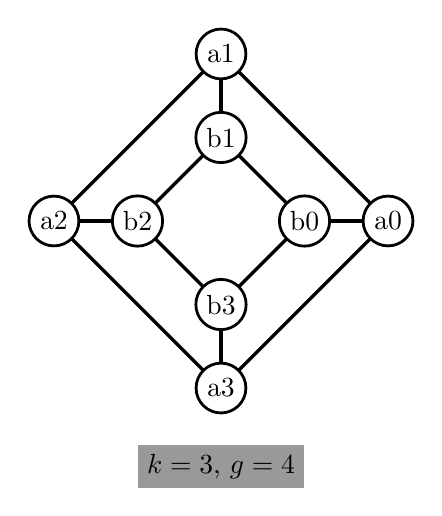
\begin{tikzpicture}
        \pgfmathsetmacro{\rada}{3*sqrt(2)/2}
        \pgfmathsetmacro{\radb}{3*sqrt(2)/4}
        \pgfmathsetmacro{\radc}{-3*sqrt(2)/2-1} 
        \grCubicalGraph[RA=\rada,RB=\radb]
        \graphcaption{0}{\radc}{$k=3$, $g=4$}
      \end{tikzpicture}
    \end{center}
  \end{minipage}
  \pause
  \begin{minipage}{0.45\linewidth}
    \begin{center}
      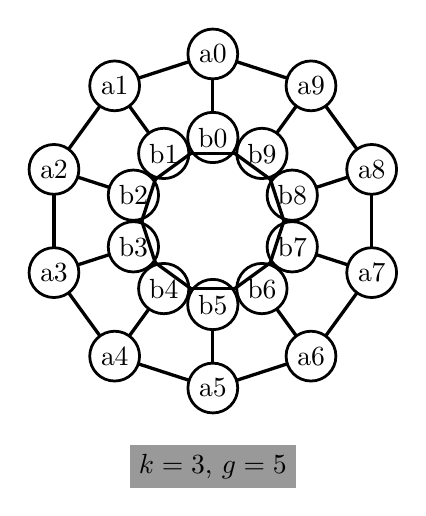
\begin{tikzpicture}
        \pgfmathsetmacro{\rada}{3*sqrt(2)/2}
        \pgfmathsetmacro{\radb}{3*sqrt(2)/4}
        \pgfmathsetmacro{\radc}{-3*sqrt(2)/2-1}
        \begin{scope}[rotate=90]
          \grDodecahedral[RA=\rada,RB=\radb]
        \end{scope}
        \graphcaption{0}{\radc}{$k=3$, $g=5$}
      \end{tikzpicture}
    \end{center}
  \end{minipage}
\end{frame}

\begin{frame}
  \begin{quote}
    \textbf{Teorema:}
    
    Para todos $k\geq3$, $g\geq3$ existe una $(k,g)$-gráfica.

    \hfill--- Sachs (1963)
  \end{quote}
\end{frame}

\begin{defnframe}{$(k,g)$-jaula}
    Una \alert{$(k,g)$-jaula} es una $(k,g)$-gráfica $G$ tal que si
    $G'$ es cualquier $(k,g)$-gráfica, entonces $|G|\leq |G'|$.  
\end{defnframe}

\begin{frame}
  \begin{teorema}
    Sea $G$ una $(k,g)$-gráfica y
    \begin{equation*}
      M(k,g)=
      \begin{cases}
        1+k+k(k-1)+\cdots+k(k-1)^{r-1}\\
        \qquad\text{si $g=2r+1$}\\
        2+2(k-1)+\cdots+2(k-1)^{r-1}\\ \qquad\text{si $g=2r$}\\
      \end{cases}
    \end{equation*}
    entonces $|G|\geq M(k,g)$.
  \end{teorema}
\end{frame}

\begin{frame}
  \begin{center}
    \begin{tikzpicture}
      \graphcaption{1.5}{4}{$k=3$, $g=4$}
      \useasboundingbox (-1,-1) rectangle (4,4);
      \VertexM[xa=0.5,ya=0,xb=0,yb=3,shows=1,starts=5,stops=14]{y0}
      \VertexM[xa=2.5,ya=0,xb=3,yb=0,shows=1,starts=5,stops=14]{x2}
      \only<1->{\Edge(y0)(x2)}
      \VertexM[xa=0,ya=2,xb=0,yb=0,shows=2,starts=5,stops=14]{x0}
      \VertexM[xa=1,ya=2,xb=1.5,yb=0,shows=2,starts=5,stops=14]{x1}
      \VertexM[xa=2,ya=2,xb=1.5,yb=3,shows=3,starts=5,stops=14]{y1}
      \VertexM[xa=3,ya=2,xb=3,yb=3,shows=3,starts=5,stops=14]{y2}
      \only<2->{\Edge(y0)(x0)}
      \only<2->{\Edge(y0)(x1)}
      \only<3->{\Edge(y1)(x2)}
      \only<3->{\Edge(y2)(x2)}
      \EdgeM[shows=4,starts=5,stops=14]{x0}{y1}
      \EdgeM[shows=4,starts=5,stops=14]{x0}{y2}
      \EdgeM[shows=5,starts=6,stops=14]{x1}{y2}
      \only<5->{\Edge(x1)(y1)}
      \only<14>{\graphcaption{1.5}{-1}{Única $(3,4)$-jaula}}
    \end{tikzpicture}
  \end{center}
\end{frame}

\begin{frame}
  \vspace*{-1cm}
  \begin{center}
    \begin{tikzpicture}
      \graphcaption{0}{4}{$k=3$, $g=5$}
      \useasboundingbox (-3.5,-3.5) rectangle (3.5,3.5);
      \VertexM[xa=0,ya=-3,xb=3*cos(234),yb=3*sin(234),shows=1,starts=10,stops=20]{x0}
      \VertexM[xa=-3,ya=-1,xb=3*cos(162),yb=3*sin(16),shows=2,starts=10,stops=20]{a0}
      \VertexM[xa=0,ya=-1,xb=1.5*cos(234),yb=1.5*sin(234),shows=2,starts=10,stops=20]{a1}
      \VertexM[xa=3,ya=-1,xb=3*cos(306),yb=3*sin(306),shows=2,starts=10,stops=20]{a2}
      \only<2->{\Edge(a0)(x0)}
      \only<2->{\Edge(a1)(x0)}
      \only<2->{\Edge(a2)(x0)}
      \VertexM[xa=-4,ya=1,xb=3*cos(90),yb=3*sin(90),shows=3,starts=10,stops=20]{b0}
      \VertexM[xa=-2,ya=1,xb=1.5*cos(162),yb=1.5*sin(162),shows=3,starts=10,stops=20]{b1}
      \only<3->{\Edge(a0)(b0)}
      \only<3->{\Edge(a0)(b1)}
      \VertexM[xa=-1,ya=1,xb=1.5*cos(90),yb=1.5*sin(90),shows=4,starts=10,stops=20]{c0}
      \VertexM[xa=1,ya=1,xb=1.5*cos(18),yb=1.5*sin(18),shows=4,starts=10,stops=20]{c1}
      \only<4->{\Edge(a1)(c0)}
      \only<4->{\Edge(a1)(c1)}
      \VertexM[xa=2,ya=1,xb=3*cos(18),yb=3*sin(18),shows=5,starts=10,stops=20]{d0}
      \VertexM[xa=4,ya=1,xb=1.5*cos(306),yb=1.5*sin(306),shows=5,starts=10,stops=20]{d1}
      \only<5->{\Edge(a2)(d0)}
      \only<5->{\Edge(a2)(d1)}

      \EdgeM[shows=6,starts=10,stops=20]{b0}{c0}
      \EdgeM[shows=6,starts=10,stops=20]{b0}{d0}

      \EdgeM[shows=7,starts=10,stops=20]{b1}{c1}
      \EdgeM[shows=7,starts=10,stops=20]{b1}{d1}

      \EdgeM[shows=8,starts=10,stops=20]{b1}{c1}
      \EdgeM[shows=8,starts=10,stops=20]{b1}{d1}

      \EdgeM[shows=8,starts=10,stops=20]{c0}{d1}
      \only<9->{\Edge(c1)(d0)}
      \only<20>{\graphcaption{0}{-3.5}{Única $(3,5)$-jaula}}
    \end{tikzpicture}
  \end{center}
\end{frame}


\begin{frame}
  \begin{minipage}{0.45\linewidth}
    \centering
    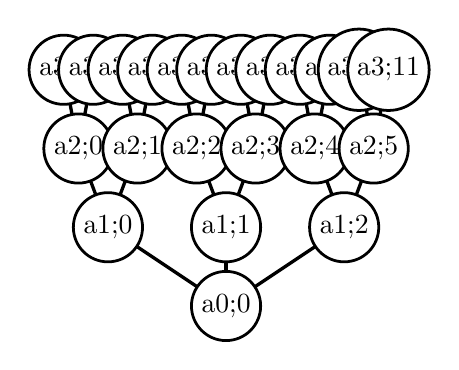
\begin{tikzpicture}
      \grSubtreeOfCage[RA=1.5,RB=1]{3}{7}
    \end{tikzpicture}
    \bigskip

    Caso impar: $1+3+3\cdot 2+3\cdot 2^{2}$.
  \end{minipage}
  \pause
  \begin{minipage}{0.45\linewidth}
    \centering
    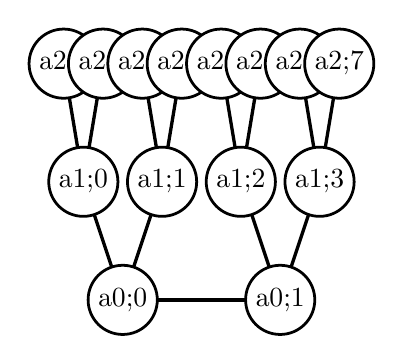
\begin{tikzpicture}
      \grSubtreeOfCage[RA=2,RB=1.5]{3}{6}
    \end{tikzpicture}
    \bigskip

    Caso par:\\ $2 + 2\cdot 2 + 2\cdot 2^{2}$.
  \end{minipage}
\end{frame}

\begin{defnframe}{gráfica de Moore}
  Si $G$ es una~$(k,g)$-gráfica con~$M(k,g)$ vértices, decimos que~$G$
  es una \alert{gráfica de Moore}.
\end{defnframe}

\begin{frame}
  \begin{teorema}
    \begin{columns}
      \begin{column}{0.72\textwidth}
        Existe una gráfica de Moore si y sólo si:
        \begin{itemize}
        \item<+-> $k=2$, $g\geq 3$ (ciclos)
        \item<+-> $g=3$, $k\geq 2$ (gráficas completas)
        \item<+-> $g=4$, $k\geq 2$ (bipartitas completas)
        \item<+-> $g=5$,
          \begin{itemize}
          \item<+-> $k=3$ (Petersen),
          \item<+-> $k=7$ (Hoffman-Singleton),
          \item<+-> $k=57$ (posiblemente).
          \end{itemize}
        \item<+-> $g=6,8,12$, y existe un $\frac{g}{2}$-gono
          generalizado de orden $k-1$.
        \end{itemize}
      \end{column}
      \begin{column}{0.23\textwidth}
        \begin{center}
          \only<1>{%
          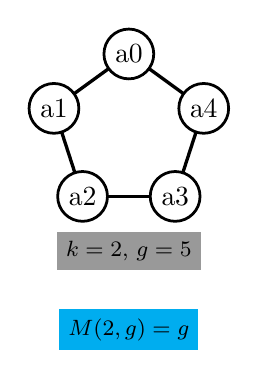
\begin{tikzpicture}
            \grCycle[RA=1.0,rotation=90]{5}
            \graphcaption{0}{-1.5}{\footnotesize $k=2$, $g=5$}
            \graphcaption[cyan]{0}{-2.5}{\footnotesize $M(2,g)=g$}
          \end{tikzpicture}
          }
          \only<2>{%
          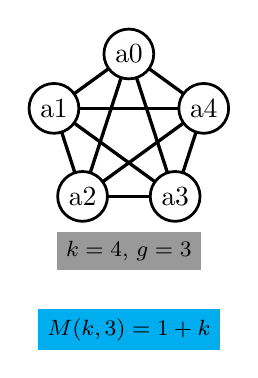
\begin{tikzpicture}
            \grComplete[RA=1.0,rotation=90]{5}
            \graphcaption{0}{-1.5}{\footnotesize $k=4$, $g=3$}
            \graphcaption[cyan]{0}{-2.5}{\footnotesize $M(k,3)=1+k$}
          \end{tikzpicture}
          }
          \only<3>{%
            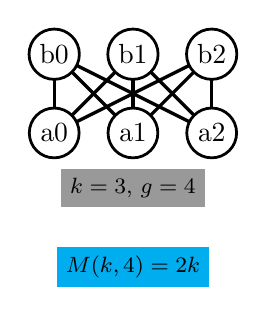
\begin{tikzpicture}
              \grCompleteBipartite[RA=1.0,RB=1.0,RS=1]{3}{3}
              \graphcaption{1.0}{-0.7}{\footnotesize $k=3$, $g=4$}
              \graphcaption[cyan]{1.0}{-1.7}{\footnotesize $M(k,4)=2k$}
            \end{tikzpicture}
          }
          \only<5>{%
            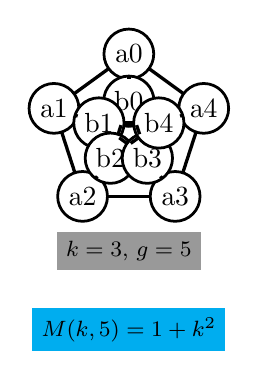
\begin{tikzpicture}
              \begin{scope}[rotate=90]
                \grPetersen[RA=1.0,RB=0.4]
              \end{scope}
              \graphcaption{0}{-1.5}{\footnotesize $k=3$, $g=5$}
              \graphcaption[cyan]{0}{-2.5}{\footnotesize $M(k,5)=1+k^{2}$}
            \end{tikzpicture}
          }
          \only<8>{%
            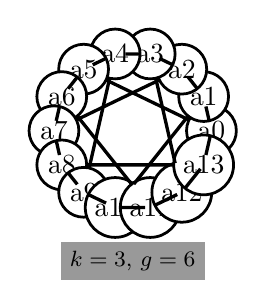
\begin{tikzpicture}
              \begin{scope}
                \grHeawood[RA=1.0]
              \end{scope}
              \graphcaption{0}{-1.65}{\footnotesize $k=3$, $g=6$}
            \end{tikzpicture}
          }
        \end{center}
    \end{column}
    \end{columns}
  \end{teorema}
\end{frame}

\begin{frame}
  \begin{center}
    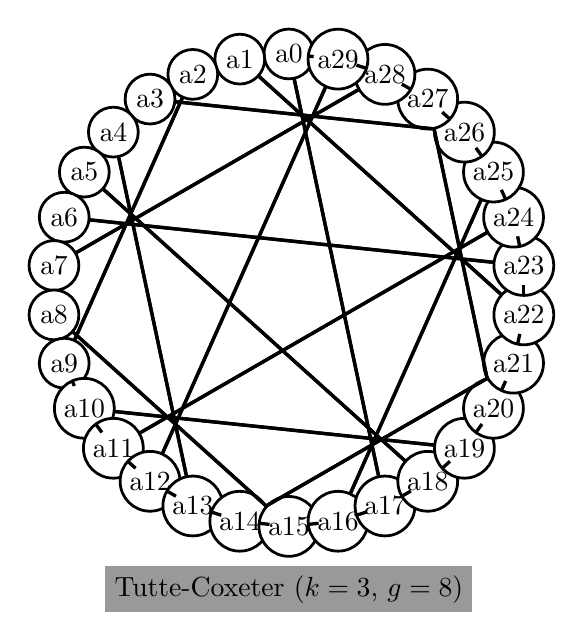
\begin{tikzpicture}
      \grTutteCoxeter[rotation=90,RA=3]
      \graphcaption{0}{-3.8}{Tutte-Coxeter ($k=3$, $g=8$)}
    \end{tikzpicture}
  \end{center}
\end{frame}

\begin{frame}
  \begin{columns}
    \begin{column}{0.55\textwidth}
      No existe una $(7,3)$-gráfica $G$ con $M(7,3)=22$ vértices.

      \uncover<2->{Sea $x$ un vértice de una tal~$G$. }
      \uncover<3->{Contemos la cantidad de $7$-ciclos que incluyen a
        $x$. }
      \uncover<4->{Hay exactamente uno por cada arista entre vértices
        marcados. }
      \uncover<7->{Por lo tanto, hay $\frac{12\cdot 2}{2}=12$
        $7$-ciclos pasando por~$x$. }
      \uncover<8->{Lo cual da $\frac{22\cdot 12}{7}$ $7$-ciclos en total.}
    \end{column}
    \begin{column}{0.42\textwidth}
      \begin{center}
        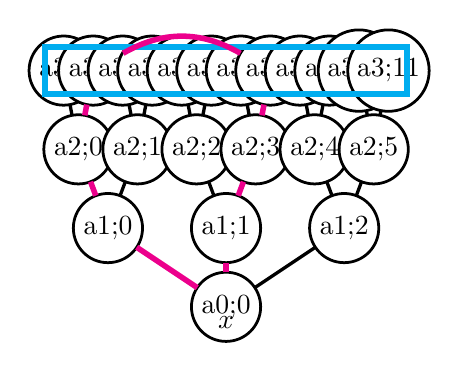
\begin{tikzpicture}
          \uncover<2->{\grSubtreeOfCage[RA=1.5,RB=1]{3}{7}}
          \uncover<2->{\draw (a0;0) node [below] {$x$};}
          \uncover<4->{\draw[line width=2pt,cyan] (-2.3,2.7) rectangle
            (2.3,3.3);}
          \uncover<5->{\Edge[local,lw=2pt,color=magenta,style={bend
              left}](a3;1)(a3;7)}
          \uncover<6->{\Edges[local,lw=2pt,color=magenta](a0;0,a1;0,a2;0,a3;1)}
          \uncover<6->{\Edges[local,lw=2pt,color=magenta](a0;0,a1;1,a2;3,a3;7)}
        \end{tikzpicture}
      \end{center}
    \end{column}
  \end{columns}
\end{frame}

\begin{frame}
  Sea $n(k,g)$ la cantidad de vértices de una $(k,g)$-jaula.

  \pause\bigskip

  Por ejemplo, $n(k,g)=M(k,g)$ si y sólo si hay una $(k,g)$ gráfica de
  Moore.

  \pause\bigskip

  Por lo que acabamos de ver, $n(3,7)>22$.

  \pause\bigskip

  Por el \alert{teorema fundamental de la teoría de gráficas},
  $n(3,7)\neq 23$.

  \pause\bigskip

  Es decir, $n(3,7)\geq 24$.
\end{frame}


\begin{frame}
  \begin{center}
    \vspace*{-1cm}
    \begin{tikzpicture}[scale=0.8]
      \useasboundingbox (-5.5,-4.5) rectangle (5.5,4.5);
      \MVert{0}{-4}{0}
      \MVert{-4}{-2}{1}
      \MVert{0}{-2}{12}
      \MVert{4}{-2}{23}
      \MVert{-5}{0}{2}
      \MVert{-3}{0}{8}
      \MVert{-1}{0}{11}
      \MVert{1}{0}{13}
      \MVert{3}{0}{16}
      \MVert{5}{0}{22}
      \MVert{-5.5}{2}{3}
      \MVert{-4.5}{2}{19}
      \MVert{-3.5}{2}{7}
      \MVert{-2.5}{2}{9}
      \MVert{-1.5}{2}{4}
      \MVert{-0.5}{2}{10}
      \MVert{0.5}{2}{14}
      \MVert{1.5}{2}{20}
      \MVert{2.5}{2}{15}
      \MVert{3.5}{2}{17}
      \MVert{4.5}{2}{5}
      \MVert{5.5}{2}{21}
      \MVert{-2}{4}{6}
      \MVert{2}{4}{18}
      \only<1->{\Edge(a0)(a1)}
      \only<1->{\Edge(a0)(a12)}
      \only<1->{\Edge(a0)(a23)}
      \only<1->{\Edge(a1)(a2)}
      \only<1->{\Edge(a1)(a8)}
      \only<1->{\Edge(a12)(a11)}
      \only<1->{\Edge(a12)(a13)}
      \only<1->{\Edge(a23)(a16)}
      \only<1->{\Edge(a23)(a22)}
      \only<1->{\Edge(a2)(a3)}
      \only<1->{\Edge(a2)(a19)}
      \only<1->{\Edge(a8)(a7)}
      \only<1->{\Edge(a8)(a9)}
      \only<1->{\Edge(a11)(a4)}
      \only<1->{\Edge(a11)(a10)}
      \only<1->{\Edge(a13)(a14)}
      \only<1->{\Edge(a13)(a20)}
      \only<1->{\Edge(a16)(a15)}
      \only<1->{\Edge(a16)(a17)}
      \only<1->{\Edge(a22)(a5)}
      \only<1->{\Edge(a22)(a21)}
      \only<2->{\Edge(a6)(a18)}
      \only<2->{\Edge(a6)(a5)}
      \only<2->{\Edge(a6)(a7)}
      \only<2->{\Edge(a18)(a19)}
      \only<2->{\Edge(a18)(a17)}
      \MEdge{3}{4}
      \MEdge[40]{3}{15}
      \MEdge{19}{20}
      \MEdge{7}{14}
      \MEdge{9}{10}
      \MEdge[40]{9}{21}
      \MEdge[40]{4}{5}
      \MEdge{10}{17}
      \MEdge{14}{15}
      \MEdge{20}{21}
      \only<16>{\graphcaption{0}{-5}{Única $(3,7)$-jaula:
          \alert{gráfica de McGee}}}
    \end{tikzpicture}
  \end{center}
\end{frame}

\begin{frame}
  Consideremos el caso $k=3$

  \begin{center}
    \begin{tabular}{cccc}
      \toprule
      $g$ & $M(3,g)$ & $n(3,g)$ & Cantidad de jaulas\\
      \midrule
      7 & 22 & 24 & 1\\
      \pause
      9 & 46 & 58 & 18\\
      \pause
      10 & 62 & 70 & 3\\
      \pause
      11 & 94 & 112 & 1\\
      \bottomrule
    \end{tabular}

    \pause\bigskip

    Para ningún otro $g\geq13$ se conoce el valor de $n(3,g)$.
  \end{center}
\end{frame}


\begin{frame}
  Sea $\rec(k,g)$ la cantidad de vértices de la menor $(k,g)$-gráfica 
  conocida. 

  \pause\bigskip 

  \begin{center}
    \begin{tabular}{cccc}
      \toprule
      $g$ & $M(3,g)$ & $n(3,g)$ & $\rec(3,g)$\\
      \midrule
      13 & 190 & $\geq 202$ & 272\\
      \pause
      14 & 254 & $\geq 260$ & 384\\
      \pause
      15 & 382 & $\geq 384$ & 620\\
      \pause
      16 & 510 &  & 960\\
      17 & 766 &  & 2176\\
      18 & 1022 & & 2640\\
      \bottomrule
    \end{tabular}
  \end{center}
\end{frame}

\begin{frame}
\begin{center}
\vspace*{-1cm}
Tabla de resultados

\bigskip

\begin{tabular}{|c|c|c|c|c|c|}
\toprule
 $k$/$g$  &  5            &  6            &            7  &  8              &            9  \\
\midrule
         3  &  \alert{10} &\alert{14}&\alert{24} (22) &\alert{30}  & \alert{58} (46)  \\
         4  &  \alert{19} (17)&\alert{26}&\textbf{67} (53)&  \alert{80} & 275 (161)  \\
         5  &  \alert{30} (26)  &  \alert{42}  &  152 (106)  &  \alert{170}   &               \\
         6  &  \alert{40} (37)  &  \alert{62}  &  294 (187)  &  \alert{312}   &               \\
         7  &  \alert{50}  &  \alert{90} (86) &               &                 &               \\
         8  &  80 (65)       &  \alert{114} &               &  \alert{800}   &               \\
         9  &  98 (82)       &  \alert{146} &               &  \alert{1170}  &               \\
\bottomrule
\end{tabular}
\end{center}

\end{frame}

\begin{imageframervf}{paper}

\end{imageframe}

\begin{frame}
  \setbeamerfont{enumerate item}{size=\large}
  Proceso para construir $(k,g)$-gráficas, comenzando por una gráfica
  dada.

  \bigskip

  \begin{scriptsize}
    \begin{enumerate}
    \item \texttt{mientras haya vértices de grado $<k$}
    \item \texttt{ { }{ }{ }mientras haya aristas ``disponibles''}
    \item \texttt{ { }{ }{ } { }{ }{ }para cada arista ``disponible''}
    \item \texttt{ { }{ }{ } { }{ }{ }  { }{ }{ }%
        calcula la suma de los grados de sus vértices}
    \item \texttt{ { }{ }{ } { }{ }{ }%
        escoge la arista con suma mayor, al azar si hay empates}
    \item \texttt{ { }{ }{ } { }{ }{ }añade la arista escogida}
    \item \texttt{ { }{ }{ }si todos los vértices tienen grado $k$}
    \item \texttt{ { }{ }{ } { }{ }{ }salva la gráfica, terminamos}
    \item \texttt{ { }{ }{ }quita 1,2 o 3 aristas}
    \end{enumerate}
  \end{scriptsize}
\end{frame}

\begin{frame}
  \vspace*{-0.5cm}
  \begin{center}
    \begin{tikzpicture}
      \MVerte{0}{0}{0}
      \MVerte{1}{4}{1}
      \MVerte{-1}{4}{2}
      \MVerte{-3}{4}{3}
      \MVerte{-5}{4}{4}
      \MVerte{-4}{0}{5}
      \MVerte{0}{-4}{6}
      \MVerte{4}{0}{7}
      \MVerte{5}{4}{8}
      \MVerte{3}{4}{9}

      \uncover<2->{\Edge(a6)(a7)}
      \uncover<3->{\Edge(a6)(a5)}
      \uncover<4->{\Edge(a6)(a0)}
      \uncover<5->{\Edge(a5)(a4)}
      \uncover<6->{\Edge(a5)(a3)}
      \uncover<7->{\Edge(a0)(a1)}
      \uncover<8->{\Edge(a0)(a2)}
      \uncover<9->{\Edge(a7)(a9)}
      \uncover<10->{\Edge(a7)(a8)}
    \end{tikzpicture}
  \end{center}
\end{frame}

\begin{frame}
  Se ha implementado el proceso anterior, usando como base el programa
  \textsf{Sage} (\texttt{http://www.sagemath.org}).
  \begin{center}
    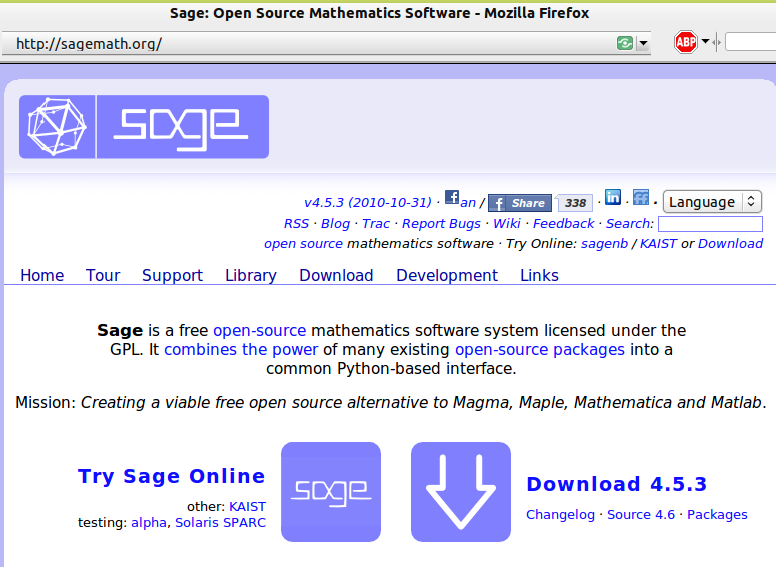
\includegraphics[height=6cm]{sagepage}
  \end{center}
\end{frame}

\begin{frame}[fragile]
  Para hacer una lista de aristas posibles:

  \bigskip
  
  \begin{minted}[fontsize=\scriptsize]{python}
def EdgeValidInCage(X,e,g,k):
    """Checks if the XEdge e could be added to X and still have a
    (k,g)-graph.
    """
    G = X.graph()
    e0 = e.ends[0]
    e1 = e.ends[1]
    return G.distance(e0,e1) >= g-1 and max([G.degree(e0),G.degree(e1)]) < k    
  \end{minted}
\end{frame}

\begin{frame}[fragile]
  Para escoger aristas a añadir:

  \bigskip
  
  \begin{minted}[fontsize=\scriptsize]{python}
def DegreeSumMax(X,edgelist,ntry):
    """Returns the edge with maximum degree sum of its extremes.
    """
    edgewithsums = sorted(edgelist,\
                              key=lambda e:degreeSum(X,e),reverse=True)
    return edgewithsums[0]
  \end{minted}
\end{frame}

\begin{frame}[fragile]
  Para aumentar aristas sucesivamente a una gráfica:

  \bigskip
  
  \begin{minted}[fontsize=\scriptsize]{python}
def ExtendXGraph(X,selectf,addf,ntry):
    """Extend an XGraph according to some method.
    """
    m = X.graph().size()
    XGraphWithEdgeAdded(X,selectf,addf,ntry)
    while X.graph().size() > m:
        m = m+1
        XGraphWithEdgeAdded(X,selectf,addf,ntry)
  \end{minted}
\end{frame}

\begin{frame}
  ver el programa\dots
\end{frame}

\begin{frame}
  \begin{center}
    \fdsfamily Hecha con software libre
    
    \bigskip

    \begin{tighttabular}{@{}c@{}c@{}c@{}c@{}c@{}c@{}}
      \gnu&\tux&\tex&\ema\\
      \pyt&\ubu&\sag&\git\\
    \end{tighttabular}

    \bigskip

    GNU \textbullet{} Linux \textbullet{} \TeX \textbullet{} Emacs\\
    Python \textbullet{} Ubuntu \textbullet{} Sage \textbullet{} Git\\
    beamer \textbullet{} AucTeX \textbullet{} org-mode
  \end{center}
\end{frame}

\begin{wordframe}
  gracias
\end{wordframe}

\end{document}

%%% Local Variables:
%%% LaTeX-command: "latex -shell-escape"
%%% End:
